%% LyX 1.1 created this file.  For more info, see http://www.lyx.org/.
%% Do not edit unless you really know what you are doing.
\documentclass[a4paper,english]{article}
\usepackage[T1]{fontenc}
\usepackage[latin1]{inputenc}
\usepackage{babel}
\usepackage{graphics}

\makeatletter

%%%%%%%%%%%%%%%%%%%%%%%%%%%%%% LyX specific LaTeX commands.
\providecommand{\LyX}{L\kern-.1667em\lower.25em\hbox{Y}\kern-.125emX\@}

%%%%%%%%%%%%%%%%%%%%%%%%%%%%%% Textclass specific LaTeX commands.
 \usepackage{GECCO_proceedings2e}

%%%%%%%%%%%%%%%%%%%%%%%%%%%%%% User specified LaTeX commands.


\makeatother
\begin{document}

\vfill{}
\title{Genetic Programming: Analysis of the Behavior of a Hardware Implementation
of GP using FPGAs and Handel-C}
\vfill{}


\author{The Author\\
Address part 1\\
Address part2\\
email@someplace +00 00 00 00 00 00}

\maketitle
\begin{abstract}
This paper analyses the behavior of a hardware implementation of Genetic
Programming using Field Programmable Gate Arrays. Three crossover
operators that limit the lengths of programs are analyzed. A truncating
operator, a limiting operator that constrains the lengths of both
offspring and a limiting operator that only constrains the length
of one offspring. The latter has some interesting properties that
suggest a new method of limiting code growth in the presence of fitness.
\end{abstract}

\section{Introduction}

Previous work has described an implementation of Genetic Programming
using Field Programmable Arrays and a high level language to hardware
compilation system called Handel-C \cite{martin:2001:gpem}. This
was tested using the XOR and symbolic regression problems. Further
work described a pipelined implementation that improved the performance
and demonstrated that the technique could be used to solve the artificial
ant problem \cite{martin-csm353:2002}. In both cases the work concentrated
on the implementation issues and increasing the clock speed of the
implementation, but put to one side the study of the behavior of the
system with respect to standard GP. Now that the raw throughput issues
have been considered it is time to look at the behavior, and investigate
and analyze some alternative implementation issues.

Because of limited hardware resources in an FPGA and to keep the design
simple and therefore efficient, the maximum program size is fixed.
To ensure that crossover always generate programs that are shorter
than the maximum, the crossover operator limits the program size by
truncating programs that exceed the fixed maximum. The effect of this
decision is investigated in this paper and then some other alternative
methods of limiting program length are explored.

The paper begins with a brief description of the implementation of
a GP system using FPGAs. This is followed by an analysis of the crossover
operator, with comparisons to standard GP systems. We then consider
two alternative crossover operators and analyze their behavior. The
analysis is then discussed and finally some further work is suggested
and some conclusions are given.


\section{A Hardware Implementation of GP using FPGAs}

For a review of previous work using FPGAs in Evolutionary Computing
refer to \cite{martin:2001:gpem}.


\subsection{Description of Handel-C}

Handel-C is a high level language that is at the heart of a hardware
compilation system known as Celoxica DK1 \cite{Celoxica:website}
which is designed to compile programs written in a C-like high level
language into synchronous hardware. The output from Handel-C is used
to create the configuration data for the FPGA. A description of the
process used by Handel-C to transform a high level language into hardware
and examples of the hardware generated can be found in \cite{page:1996}.
Handel-C has its roots in CSP and Occam.

The C-like syntax makes the tool appealing to software engineers with
little or no experience of hardware. They can quickly translate a
software algorithm into hardware, without having to learn about VHDL
or FPGAs in detail. Handel-C has extended the C syntax to support
the parallelization of code.


\subsection{Target Hardware}

The target hardware for this work is a Celoxica RC1000 FPGA development
board fitted with a Xilinx XCV2000E Virtex-E FPGA \cite{Xilinx:2001}
having 43,200 logic cells and 655,360 bits of block RAM, a PCI bridge
that communicates between the RC1000 board and the host computer's
PCI bus, and four banks of static RAM.


\subsection{Program Representation}

Handel-C does not support a stack, which means that a standard tree
based representation is not straightforward to implement because recursion
is not supported by the language. An alternative to a tree representation
is a linear representation which has been used by others to solve
some hard GP problems \cite{Nordin:1995:tcp}. Using a linear representation,
a program consists of a sequence of words which are interpreted by
the problem specific fitness function. 


\section{Analysis of the Hardware Implementation}

The hardware design uses a linear program representation with a fixed
maximum size. The choice of a fixed maximum size was made to make
the storage of programs in on-chip RAM and off-chip RAM efficient
and simple to implement. Consequently a method of limiting the program
size during crossover was needed. The first implementation used a
truncating crossover. This is compared to a second method of limiting
lengths, called the limiting crossover operator.


\subsection{Artificial Ant }

This popular test problem was originally described by Jefferson \cite{jefferson:1992}
and in the context of GP is described by Koza \cite{koza:book}. It
involves finding a program for an ant-like machine that enables it
to navigate its way round a trail of food on a 32x32 toroidal grid
of cells within a fixed number of time steps. In the hardware implementation
the function set \( {\cal F}=\{IF\_FOOD,\, PROGN2\} \) where \( IF\_FOOD \)
is a two argument function that looks at the cell ahead and if it
contains food evaluate the first terminal, otherwise evaluate the
second terminal. \( PROGN2 \) evaluates its first and second terminals
in sequence. The terminal set \( {\cal T}=\{LEFT,\, RIGHT,\, MOVE,\, NOP\} \),
where \( LEFT \) and \( RIGHT \) change the direction the ant is
facing, \( MOVE \) moves the ant one space forwards to a new cell,
and if the new cell contains food, the food is eaten. \( NOP \) is
a no-operation terminal and has no effect on the ant but is included
to make the number of terminals a power of 2, which simplifies the
hardware logic. Each time \( LEFT,\, RIGHT \) or \( MOVE \) is executed,
the ant consumes one time step. The run stops when either all the
time steps have been used, or the ant has eaten all the food. This
test problem was chosen because it is known to be a hard problem for
GP to solve \cite{langdon:1998:antspace}.

All the results in this section use the Santa Fe trail, which has
89 pellets of food. Each experiment was run 500 times and the average
of all the runs taken. In all cases, unless stated otherwise, the
population size is 1024, the maximum program length is 31 and all
experiments were run for 32 generations. The maximum number of time
steps for the ant to complete its trail is 1024 instead of the usual
600 time steps. This is because in order to make the logic as efficient
as possible, loop iterators in the design are required to be a power
of two. This is so that by testing the carry bit, loop termination
can be performed without the need to implement wide comparators which
can introduce significant delays into the design.


\subsection{Behavior Analysis}

The measurement of overall GP behavior is frequently limited to plotting
the average population fitness vs. generation. This is shown for the
artificial ant problem using the original hardware implementation
in Figure \ref{fig:Initial Performance}. 
\begin{figure}[htb]
{\centering \resizebox*{8cm}{4.2cm}{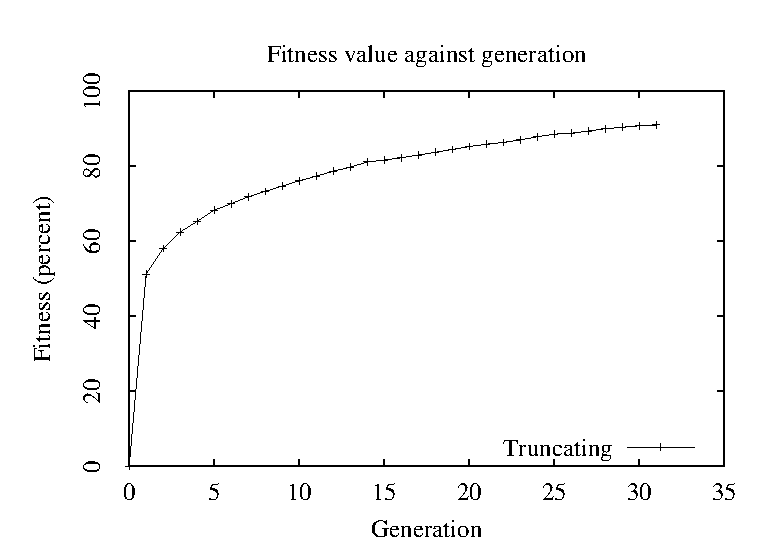
\includegraphics{images/hw_trunc_lfsr_perf.eps}} \par}


\caption{\label{fig:Initial Performance}GP Performance of the original design}
\end{figure}
This will be used as a baseline when looking at changes to the original
design. However, when looking for the reasons to explain why a feature
of an operator or representation has an effect, raw performance gives
us a very restricted view of what is happening, and more analytical
methods are needed. One such method is to consider one or more aspects
of the internal population dynamics during a run. Recently a lot of
work has been done to develop exact schema theories for Genetic Programming
\cite{poli:2001:EuroGP_general}\cite{poli:2001:EuroGP_exact}, which,
among other things, give us a description of the expected changes
in the program length distribution during a GP run. The asymptotic
distribution of program lengths is important to us because it is a
way of comparing the sampling behavior (search bias) of different
crossover operators and replacement strategies.

Two separate implementations were used during the analysis. Firstly,
a simple one that simulated the effects of crossover was used to show
the expected program length distributions in the absence of fitness.
We call this the GP simulator in this paper. Secondly, the hardware
implementation was used to obtain results both with and without fitness.

Starting with the GP simulator with a uniform initial length distribution
and ignoring the effects of fitness, Figure \ref{fig:DIST sim stdgp}
shows the expected length distribution for generations 0,1,10 and
31. In this case there is no maximum program size. This agrees with
the results in \cite{poli:2001:EuroGP_exact} where the distribution
asymptotically converges to a discrete Gamma distribution.
\begin{figure}[htb]
{\centering \resizebox*{8cm}{4.2cm}{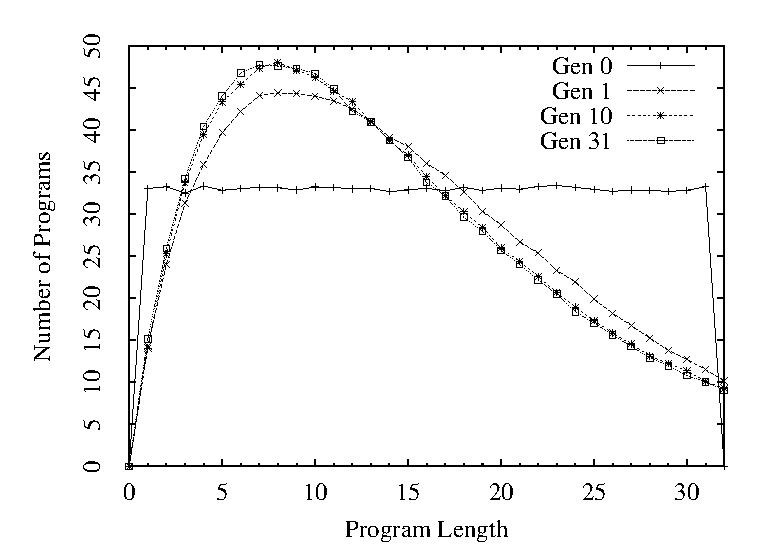
\includegraphics{images/sim_nofit_stdgp.eps}} \par}


\caption{\label{fig:DIST sim stdgp}Program length distribution for standard
GP crossover using a linear program representation, a global replacement
strategy, non-steady state and a flat fitness landscape.}
\end{figure}



\subsection{Truncating Crossover Operator}

This crossover operator ensures programs do not exceed the maximum
program length by selecting crossover points in two individuals at
random and exchanging the tail portions up to the maximum program
length. Crossovers that result in programs exceeding the maximum length
are truncated at the maximum length. This crossover operator was chosen
to minimize the amount of logic required and the number of clock cycles
needed. This is illustrated in Figure \ref{fig:Truncating crossover operator}.
\begin{figure}[htb]
{\centering \resizebox*{8cm}{4.2cm}{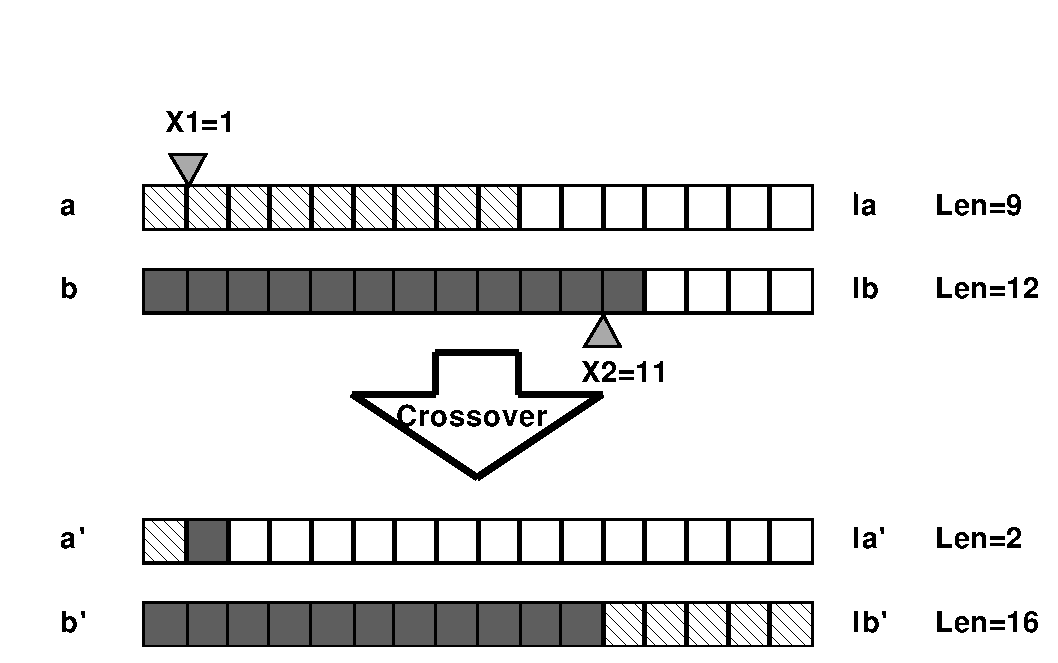
\includegraphics{images/crossover1.eps}} \par}


\caption{\label{fig:Truncating crossover operator}Truncating crossover operator}
\end{figure}
For two programs \( a \) and \( b \) that have lengths \( l_{a} \)
and \( l_{b} \), two crossover points \( x_{a} \) and \( x_{b} \)
are chosen at random so that \( 0\leq x_{a}<l_{a} \) and \( 0\leq x_{b}<l_{b} \).
The program size limit is \( L_{max} \). After crossover the new
lengths are \( l_{a}'=\min \, ((x_{a}+l_{b}-x_{b}),L_{max}) \) and
\( l_{b}'=\min \, ((x_{b}+l_{a}-x_{a}),L_{max}) \).

When the GP simulator is modified to implement the truncating crossover,
the result is shown in Figure \ref{fig:DIST sim nofit trunc} for
the flat fitness landscape case.
\begin{figure}[htb]
{\centering \resizebox*{8cm}{4.2cm}{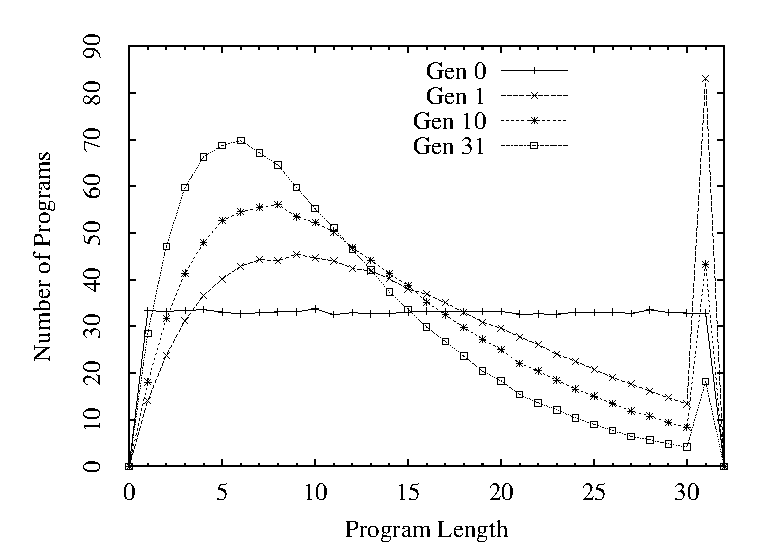
\includegraphics{images/sim_nofit_trunc.eps}} \par}


\caption{\label{fig:DIST sim nofit trunc}Program length distribution with
truncating crossover for standard GP on a flat fitness landscape.}
\end{figure}
The behavior of the hardware implementation using the truncating crossover
operator is shown in Figure \ref{fig:DIST hw nofit trunc}.
\begin{figure}[htb]
{\centering \resizebox*{8cm}{4.2cm}{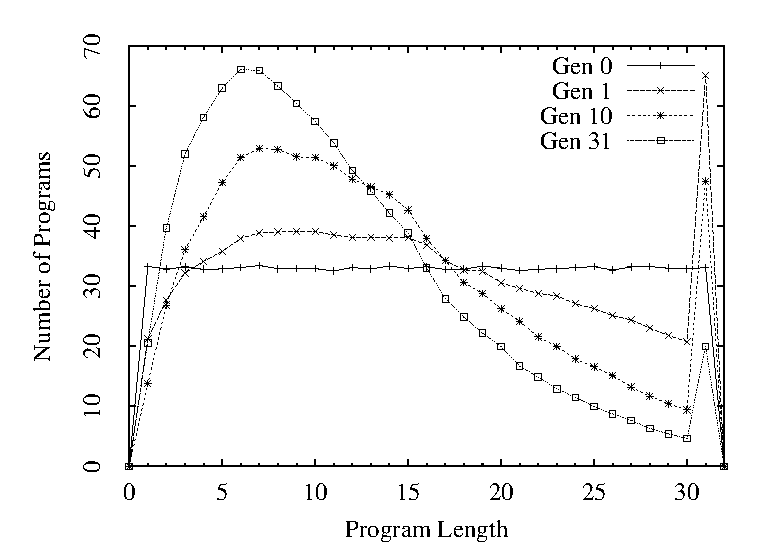
\includegraphics{images/hw_nofit_trunc.eps}} \par}


\caption{\label{fig:DIST hw nofit trunc}Program length distribution using
truncating crossover using a linear program representation on a flat
fitness landscape. From the hardware implementation.}
\end{figure}
A feature of these results is that there is initially a large peak
at the maximum program size of 31, but in subsequent generations the
distribution tends to resemble a Gamma distribution like the one in
Figure \ref{fig:DIST sim stdgp}. However, it is important to note
that it not the same Gamma distribution, because the mean program
length tends to decrease with this crossover operator. The reason
is that with the truncation the amount of genetic material removed
from the parents when creating the offspring may be bigger than the
amount of genetic material replacing it. The differences between Figures
\ref{fig:DIST sim nofit trunc} and \ref{fig:DIST hw nofit trunc}
are believed to arise because the simulator uses generational GP,
while the hardware implementation uses steady state GP.

When fitness is used, the length distribution changes as shown in
Figure \ref{fig:DIST hw fit trunc}, but it still retains some of
the features of a Gamma distribution. The striking feature is the
large peak at the maximum program length limit which represents 13\%
of the total population.
\begin{figure}[htb]
{\centering \resizebox*{8cm}{4.2cm}{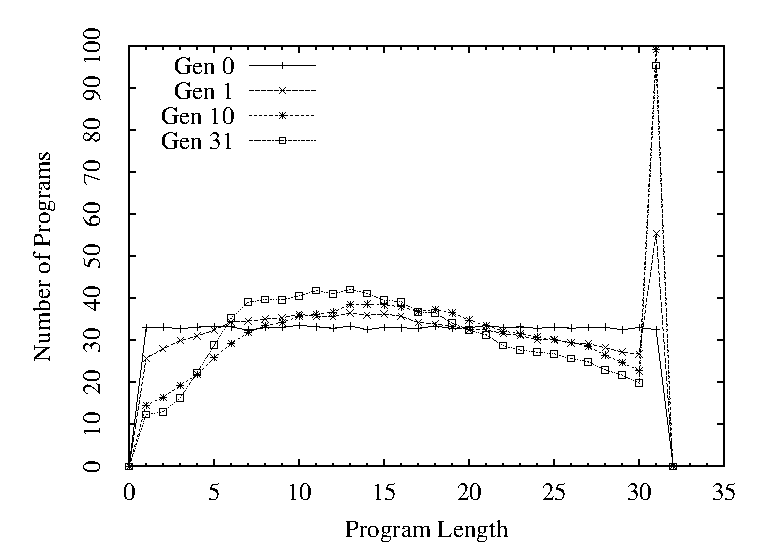
\includegraphics{images/hw_fit_trunc.eps}} \par}


\caption{\label{fig:DIST hw fit trunc}Program length distribution using truncating
crossover using a linear program representation with fitness. From
the hardware implementation.}
\end{figure}



\subsection{Limiting Crossover Operator}

An alternative method of ensuring that programs do not exceed the
fixed limit is to choose crossover points that result in programs
that are below the program size limit \( L_{max} \). For two programs
\( a \) and \( b \), with lengths \( l_{a} \) and \( l_{b} \),
two crossover points \( x_{a} \) and \( x_{b} \) are chosen so that
\( 0\leq x_{a}<l_{a} \) and \( 0\leq x_{b}<l_{b} \). After crossover
the new lengths are simply \( l_{a}'=x_{a}+l_{b}-x_{b} \) and \( l_{b}'=x_{b}+l_{a}-x_{a} \).
If \( l_{a}'>L_{max} \) or \( l_{b}'>L_{max} \) the selection of
\( x_{a} \) and \( x_{b} \) is repeated until \( l_{a}'\le L_{max} \)
AND \( l_{b}'\le L_{max} \).

This is the approach taken in lilgp when the \texttt{keep\_trying}
parameter is enabled \cite{zonger:1996:lilgp}, and other tree based
GP systems, to limit the tree depth and the total number of nodes
in a program tree. When this crossover operator is implemented in
the GP simulator the program length distribution changes, as shown
in Figure \ref{fig:DIST sim nofit limit single}. 
\begin{figure}[htb]
{\centering \resizebox*{8cm}{4.2cm}{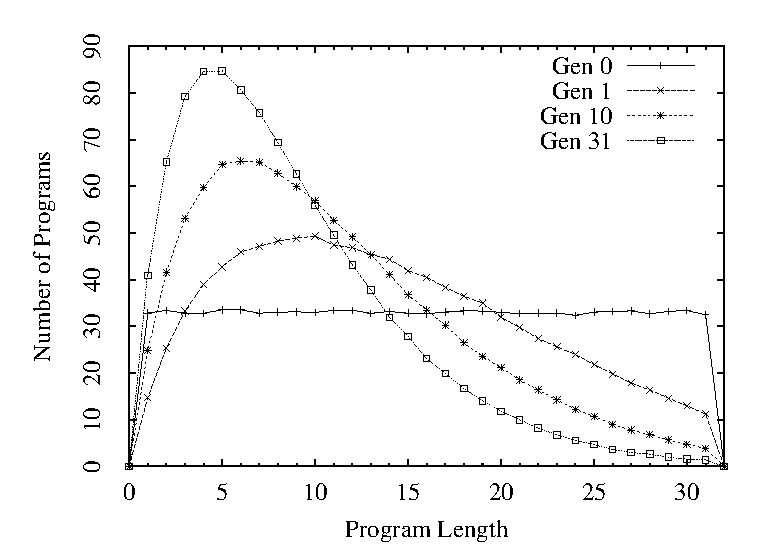
\includegraphics{images/sim_nofit_limit.eps}} \par}


\caption{\label{fig:DIST sim nofit limit single}Program length distribution
using limiting crossover operator and a global replacement strategy
on a flat fitness landscape.}
\end{figure}
A feature of this result is that the mean program length moves towards
smaller values. After 31 generations, the population size distribution
shape resembles the one produced with standard GP. 

When this method of limiting the program length was implemented in
the hardware version, we obtained the distribution shown in Figure
\ref{fig:DIST hw nofit limit dual}. In contrast to the GP simulator
the program length distribution remains reasonably static between
generations 1 and 31.
\begin{figure}[htb]
{\centering \resizebox*{8cm}{4.2cm}{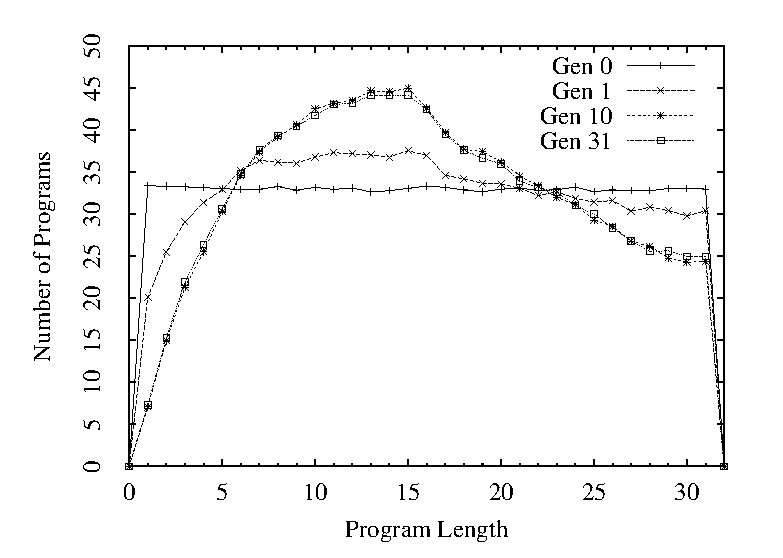
\includegraphics{images/hw_nofit_limit.eps}} \par}


\caption{\label{fig:DIST hw nofit limit dual}Program length distribution
using limiting crossover on a flat fitness landscape, from the hardware
implementation.}
\end{figure}
In an effort to understand the different behavior between the results
in Figures \ref{fig:DIST sim nofit limit single} and \ref{fig:DIST hw nofit limit dual}
it was noted that the hardware implementation required both of the
offspring programs \( a' \) AND \( b' \) to be shorter than \( L_{max} \)
but that the simulation only considered one offspring at a time, effectively
requiring \( a' \) OR \( b' \) to be shorter. The latter case is
referred to as the single-child variant in the rest of this paper,
and the original the dual-child variant. In the case of the single-child
variant, if one of the programs was larger than the maximum, it was
simply discarded and the parent substituted in its place, and if both
children were larger than the limit, the two crossover points would
be chosen again. If both children were smaller than the limit, they
would both be available as candidates in the next generation. When
the hardware implementation was modified to incorporate the single-child
variant limiting method, the result shown in Figure \ref{fig:DIST hw nofit limit single}
was obtained, closely matching that from the simulation. Again, the
difference between Figure \ref{fig:DIST sim nofit limit single} and
Figure \ref{fig:DIST hw nofit limit single} is believed to be due
to the use of steady-state GP in the hardware implementation.
\begin{figure}[htb]
{\centering \resizebox*{8cm}{4.2cm}{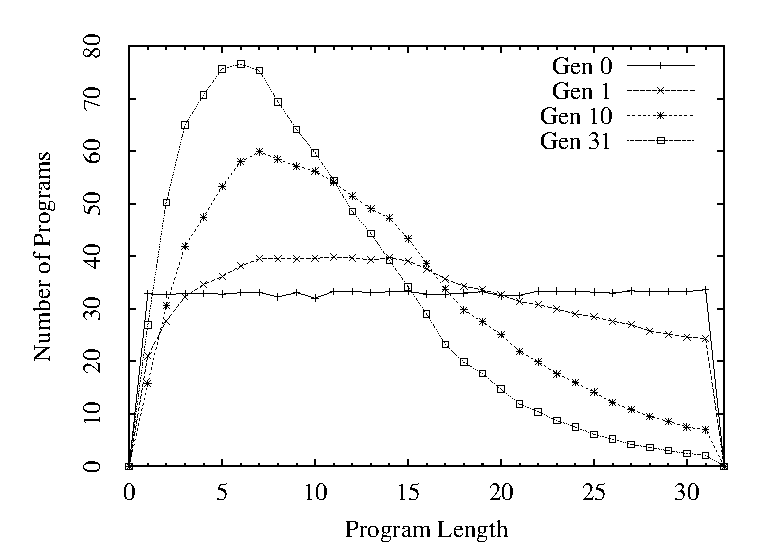
\includegraphics{images/hw_nofit_limit_single.eps}} \par}


\caption{\label{fig:DIST hw nofit limit single}Program length distribution
using limiting crossover on a flat fitness landscape and the single-child
variant. From the hardware implementation.}
\end{figure}
When fitness is enabled using the dual-child variant, there is a large
bias in favor of longer programs as shown in Figure \ref{fig:DIST hw fit limit dual}.
An interesting artifact of this graph is the sharp rise in program
lengths for generations 10 and 31 above length 15, and the plateau
after length 15. This is likely to be due to the distribution of fitness
in the program search space and can be seen as a form of what is commonly
termed bloat \cite{langdon:2000:fairxo}.
\begin{figure}[htb]
{\centering \resizebox*{8cm}{4.2cm}{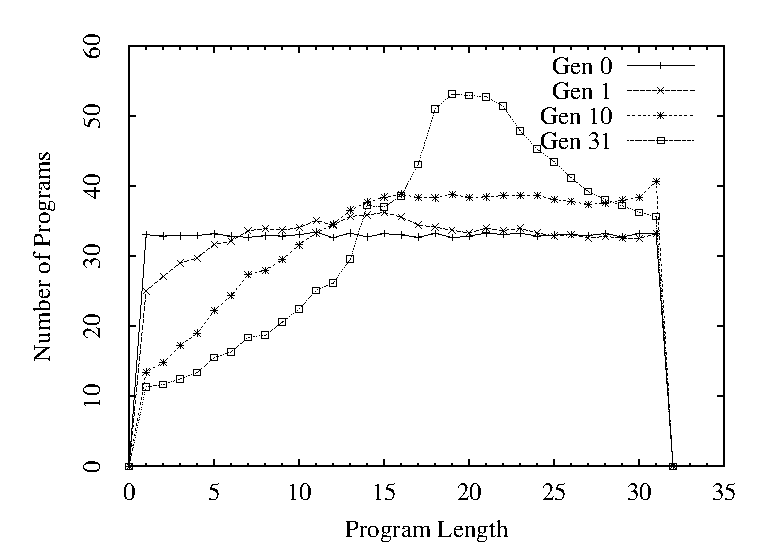
\includegraphics{images/hw_fit_limit.eps}} \par}


\caption{\label{fig:DIST hw fit limit dual}Program length distribution using
limiting crossover with fitness and the dual-child variant. From the
hardware implementation.}
\end{figure}
However, when the program length distribution using the single-child
variant was plotted, shown in Figure \ref{fig:DIST hw fit limit single},
the length distribution peaks at around the mean of \( L_{max} \).
This unexpected behavior is interesting since it appears to have avoided
the phenomenon commonly known as bloat.
\begin{figure}[htb]
{\centering \resizebox*{8cm}{4.2cm}{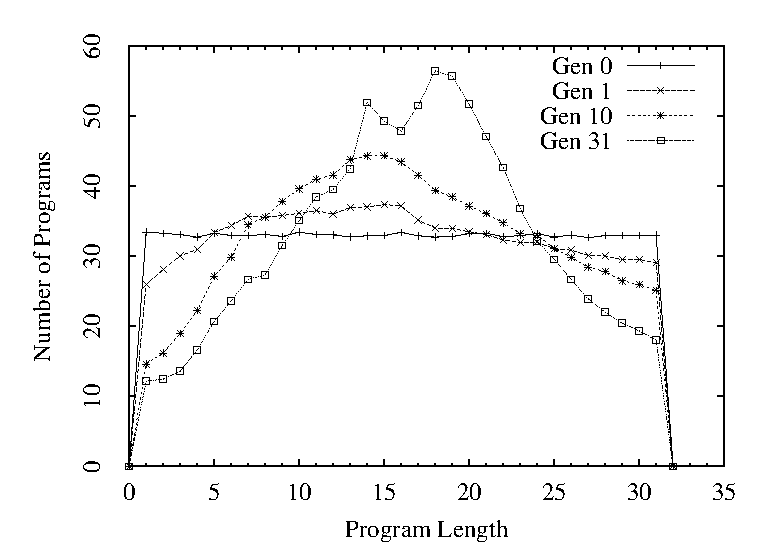
\includegraphics{images/hw_fit_limit_single-32.eps}} \par}


\caption{\label{fig:DIST hw fit limit single}Program length distribution
using limiting crossover with fitness and the single-child variant.
From the hardware implementation.}
\end{figure}


The effect of using the limiting crossover operator with and without
the single-child variant on the behavior of the system is shown in
Figure \ref{fig:PERF combined} together with the original behavior.
This graph shows that all three crossover implementations have a similar
rate of improvement, with the limiting crossover operator with single-child
variant maybe performing slightly better on the ant problem.
\begin{figure}[htb]
{\centering \resizebox*{8cm}{4.2cm}{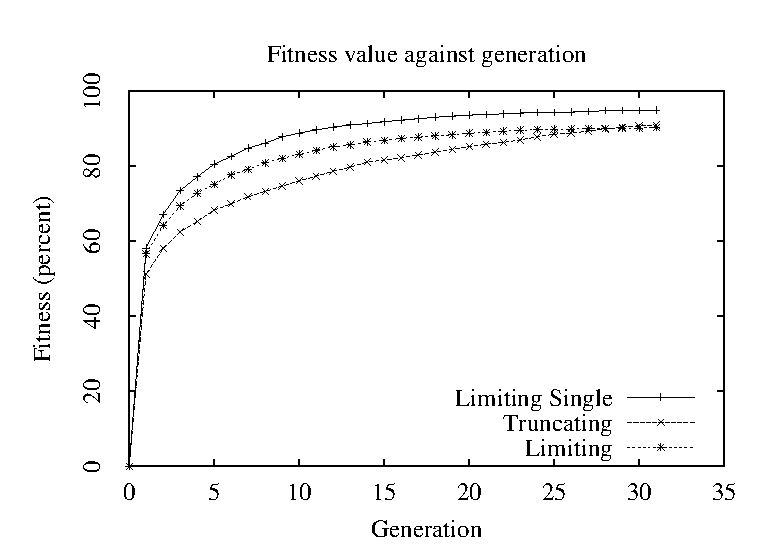
\includegraphics{images/hw_limit_lfsr_single_perf.eps}} \par}


\caption{\label{fig:PERF combined}Comparative GP behavior of the hardware
implementation for the ant problem using truncating crossover and
limiting crossover.}
\end{figure}


Finally, the distribution of 100\% correct program lengths was measured
for truncating and both limiting crossovers. The hardware implementation
was run 500 times, and if a 100\% correct program was generated, the
length was recorded. These are shown in Figures \ref{fig:LEN truncate},
\ref{fig:LEN limit dual} and \ref{fig:LEN limit single} respectively. 
\begin{figure}[htb]
{\centering \resizebox*{8cm}{4.2cm}{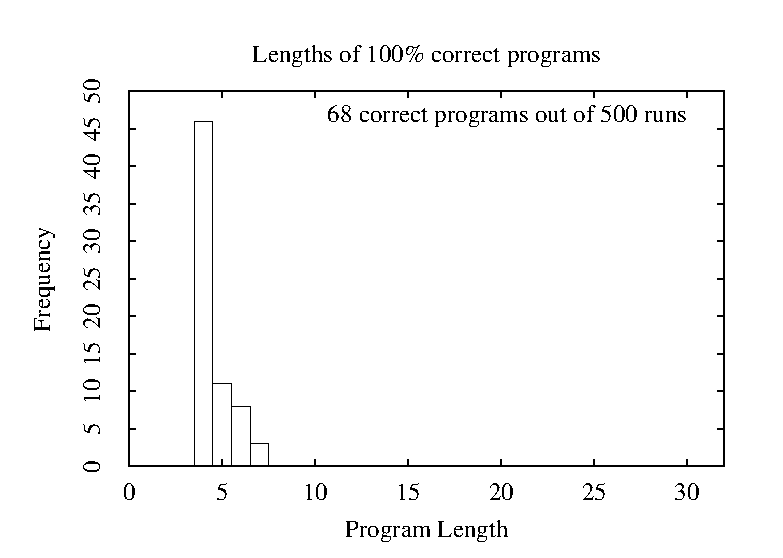
\includegraphics{images/hw_trunc_lengths.eps}} \par}


\caption{\label{fig:LEN truncate}Distribution of lengths of 100\% correct
programs using the truncating crossover operator.}
\end{figure}



\begin{figure}[htb]
{\centering \resizebox*{8cm}{4.2cm}{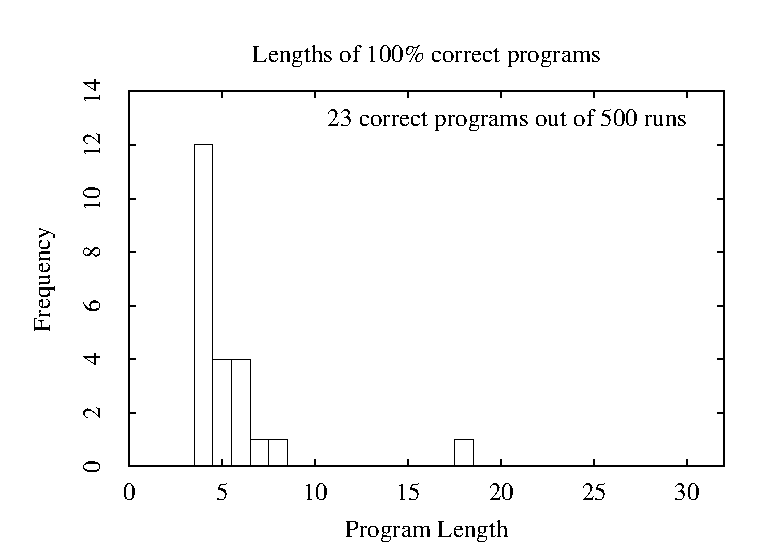
\includegraphics{images/hw_limit_lengths.eps}} \par}


\caption{\label{fig:LEN limit dual}Distribution of lengths of 100\% correct
programs using the dual-child variant limiting crossover operator.}
\end{figure}

\begin{figure}[htb]
{\centering \resizebox*{8cm}{4.2cm}{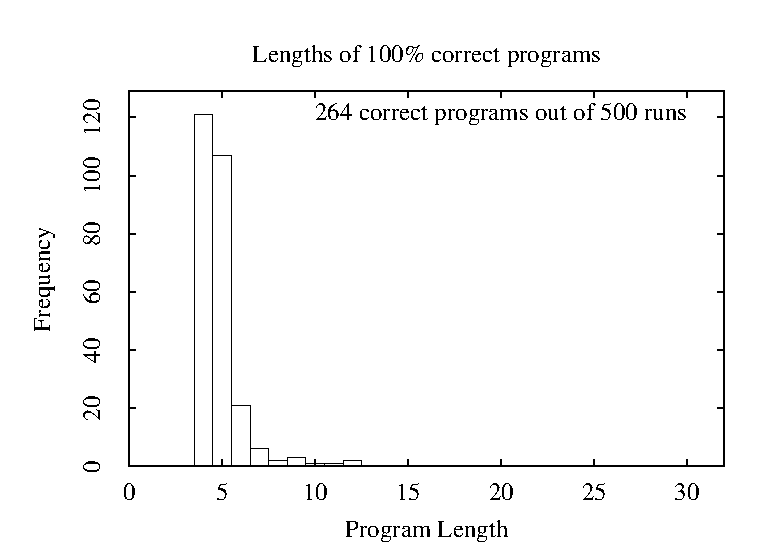
\includegraphics{images/hw_limit_lengths_single.eps}} \par}


\caption{\label{fig:LEN limit single}Distribution of lengths of 100\% correct
programs using the the single-child variant limiting crossover operator.}
\end{figure}


From these plots we can see that truncating crossover has allowed
GP to find more 100\% correct programs than the limiting crossover
using the dual-child variant. However, when using the single-child
variant, limiting crossover found the most 100\% correct programs. 

It is interesting to note that the results shown in Figure \ref{fig:PERF combined}
do not obviously show this difference in the outcome, highlighting
the weakness of using the standard measure of performance.

The results shown in Figures \ref{fig:LEN truncate},\ref{fig:LEN limit dual}
and \ref{fig:LEN limit single} suggest that for the artificial ant
problem implemented in hardware, programs of length 4 or 5 are most
likely to be correct. It was then observed that the peak program length
in Figure \ref{fig:DIST hw fit limit single} was larger than length
4. From this is was conjectured that if the maximum program length
was reduced from 32, moving the peak closer to the program length
that occurred most frequently, that GP may find even more successful
programs. Two further experiments were therefore performed using maximum
lengths of 16 and 8. The results of running the hardware implementation
with these modified lengths is shown in Figures \ref{fig:LEN limit single 16}
and \ref{fig:LEN limit single 8}.
\begin{figure}[htb]
{\centering \resizebox*{8cm}{4.2cm}{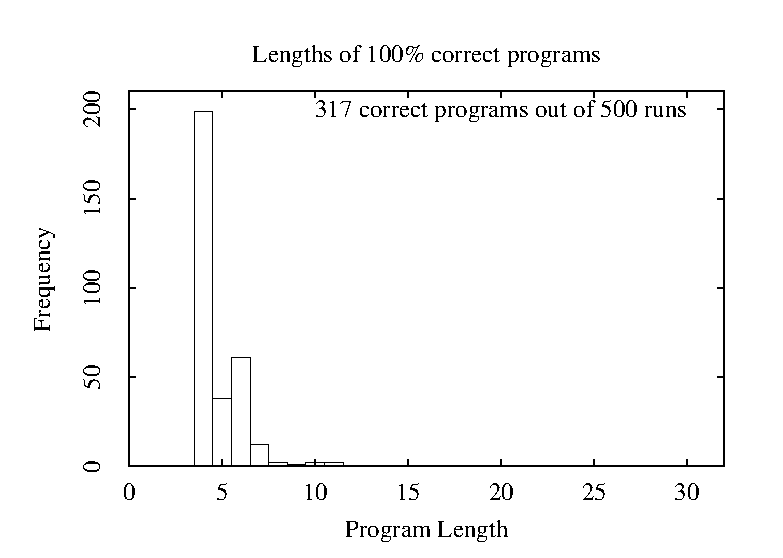
\includegraphics{images/hw_limit_lengths_single_16.eps}} \par}


\caption{\label{fig:LEN limit single 16}Distribution of lengths of 100\%
correct programs using the the single-child variant limiting crossover
operator and a length limit of 16}
\end{figure}

\begin{figure}[htb]
{\centering \resizebox*{8cm}{4.2cm}{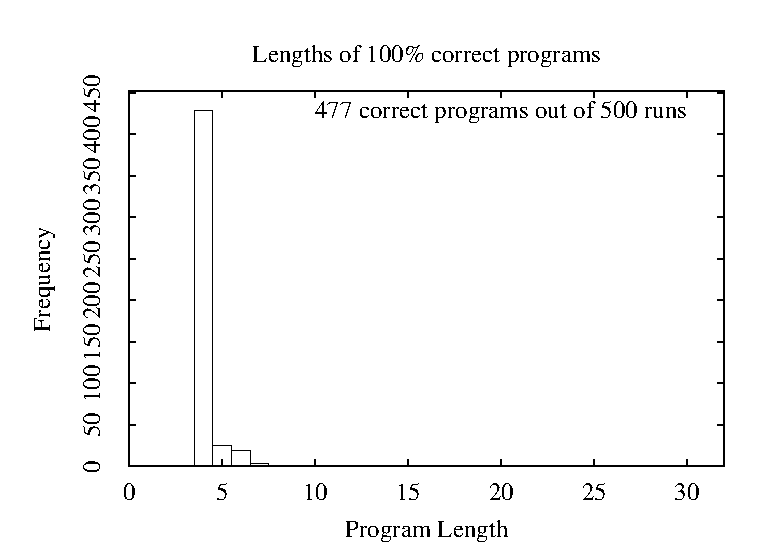
\includegraphics{images/hw_limit_lengths_single_8.eps}} \par}


\caption{\label{fig:LEN limit single 8}Distribution of lengths of 100\% correct
programs using the the single-child variant limiting crossover operator
and a length limit of 8}
\end{figure}
This confirmed the idea that, by limiting the program lengths that
GP is allowed to create, that GP produced more 100\% correct programs.
The corresponding program length distributions are shown in Figures
\ref{fig:DIST hw fit limit single 16} and \ref{fig:DIST hw fir limit single 8}.
These both have similar characteristics to Figure \ref{fig:DIST hw fit limit single}
and show that the program length distribution peaks close to the peak
of the successful programs.
\begin{figure}[htb]
{\centering \resizebox*{8cm}{4.2cm}{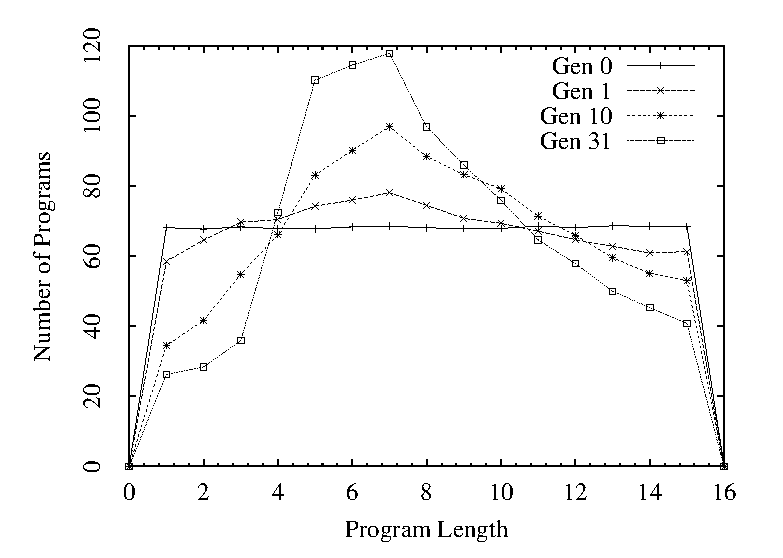
\includegraphics{images/hw_fit_limit_single-16.eps}} \par}


\caption{\label{fig:DIST hw fit limit single 16}Program length distribution
using limiting crossover with fitness and the single-child variant.
Maximum length limited to 16. From the hardware implementation.}
\end{figure}

\begin{figure}[htb]
{\centering \resizebox*{8cm}{4.2cm}{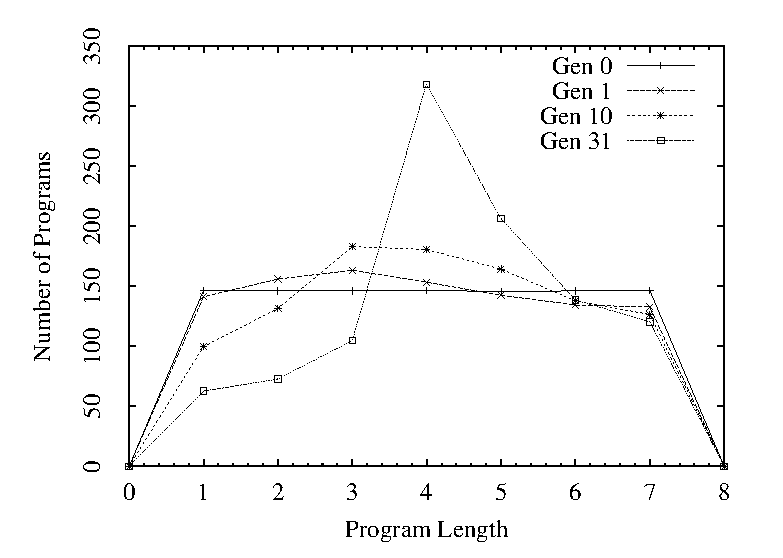
\includegraphics{images/hw_fit_limit_single-8.eps}} \par}


\caption{\label{fig:DIST hw fir limit single 8}Program length distribution
using limiting crossover with fitness and the single-child variant.
Maximum length limited to 8. From the hardware implementation.}
\end{figure}



\section{Discussion}

The differences between the dual-child and single-child variants can
be explained by considering first the dual-child case. Starting with
a uniform distribution of program lengths \( 0<l\leq L_{max} \),
the average program length is given by \( L_{avg}=\frac{L_{max}}{2} \)
and the average crossover point is \( \frac{L_{avg}}{2} \). Every
crossover produces two offspring, the average length of which is \( \frac{L_{max}}{2} \),
with one smaller and one larger program produced. When one of the
offspring exceeds \( L_{max} \) both crossover points are re-selected
until both programs satisfy the length constraint. The result is that
the average program length using this crossover will remain \( \frac{L_{max}}{2} \).
However, in the single-child case, only one child needs to meet the
length constraint. With one long and one short offspring, the short
offspring will be more likely to satisfy the constraint and so be
selected for propagation. Because the shorter program is preferred,
the mean program length will tend to continually decrease. In summary,
in the absence of fitness, the single-child variant selects programs
that are on average smaller than \( \frac{L_{max}}{2} \). In the
presence of fitness we believe that this pressure to decrease the
mean program length competes with the well documented tendency of
GP programs to grow in the presence of fitness. The result is that
when using the single length constraint and an upper bound on the
program length, the program length distribution does not have a strong
bias to longer lengths.

A side effect of using the single child variant is that when a long
program is rejected, a copy of the parent is propagated to the next
generation. This means that even if crossover is used as the only
operator, a proportion of straightforward reproduction will be present.

A practical penalty of the limiting crossover approach is that multiple
passes may be required to obtain two crossover points that satisfy
the length constraints. Depending on the implementation this could
have an impact on the time needed to complete a GP run. In practice
for most problems the time required for crossover in a standard GP
system is much smaller than the time for evaluating programs, and
so will only extend the time required by a small factor. In the hardware
implementation, crossover is performed in parallel with evaluation,
so there will be no impact for most problems where fitness evaluation
takes longer than selection and breeding. For the artificial ant problem
implemented in hardware, the limiting crossover operators did not
have any effect on the overall performance of the design, both the
clock speed and number of clock cycles remained the same as the truncating
crossover implementation. It is worth noting that the single-child
limiting crossover will need fewer iterations to find a legal offspring,
so this will have a smaller effect on the overall performance.

The effect of adjusting the program length limit so that the peak
in the length distribution is closer to the peak of optimal program
lengths suggests that allowing programs to be unlimited in length
may be detrimental to using GP effectively. 


\section{Further work}

From the results in \cite{poli:2001:EuroGP_general} we would expect
similar behavior when these techniques are applied to standard tree
based GP, and this is currently being investigated.

Other techniques have been suggested for controlling the program size
during evolution, such as the smooth operators \cite{page:1999:smuxspmGP},
homologous and size fair operators \cite{langdon:2000:fairxo} which
could also be adapted to a hardware implementation.

So far, only one problem has been analyzed using the hardware implementation
of GP and to get a more complete picture of the effects of the design
decisions more problems need to be implemented and analyzed.


\section{Conclusions}

This analysis, based on measuring the program length distributions
was prompted by the results from the work on a general schema theory
of GP. It has led us to an implementation of crossover that allows
us to constrain the maximum program lengths. For the ant problem implemented
in hardware we have discovered a mechanism that avoids the effects
of unconstrained program growth, and indeed allows us to obtain far
more correct programs than.

In conclusion, all three crossover operators are effective in the
hardware implementation when applied to the artificial ant problem,
with the single-child limiting crossover performing ahead of the other
two. The behavior of the single-child limiting crossover in the presence
of fitness is interesting and suggests another mechanism for controlling
code growth. 


\subsubsection*{Acknowledgements}

{*} {*}{*}{*}{*}{*} {*}{*}{*}{*}{*} {*}{*}{*}{*}{*} {*}{*}{*}{*}{*}
{*}{*}{*}{*}{*} {*}{*}{*}{*}{*} {*}{*}{*}{*}{*} {*}{*}{*}{*}{*} {*}{*}{*}{*}{*}
{*}{*}{*}{*}{*} {*}{*}{*}{*}{*} {*}{*}{*}{*}{*} {*}{*}{*}{*}{*} {*}{*}{*}{*}{*} 

\bibliographystyle{abbrv}
\bibliography{handelc}

\end{document}
